\section{Calculation of the branching fraction}
\label{sec:dsphi:bf}
The branching fraction of the decay \btodsphi is determined with respect to the normalization
channel \btodsd, where $\decay{\Dz}{\Km\pip}$, using
\begin{equation}
  \BF\big(\btodsphi\big) =
  \frac{\varepsilon\big(\decay{\Bp}{\Ds\Dzb}\big)}{\varepsilon\big(\btodsphi\big)}
  \cdot
  \frac{\BF\big(\decay{\Dzb}{\Km\pip}\big)}{\BF\big(\phitokk\big)}
  \cdot
  \frac{N\big(\btodsphi\big)}{N\big(\decay{\Bp}{\Ds\Dzb}\big)}
  \cdot
  \BF\big(\btodsd\big)
  , \\
  \label{eq:dsphi:bf}
\end{equation}
where $N$ denotes a yield and $\varepsilon$ denotes an efficiency.
This choice of normalization channel means that the values of the branching fraction
$\decay{\Ds}{\kkpi}$, which has a $5\pc$ uncertainty, cancels.
%Reference~\cite{LHCb-CONF-2012-009} details an analysis including the decay \btodsd
%is measured with an --- almost --- identical selection.
%Values for the normalizaton channel were previoiusly calculated in \Ref{LHCb-CONF-2012-009}.

The signal yield of the decay \btodsphi is determined by performing an unbinned maximum likelihood
fit to the invariant mass spectrum of the candidate \Bp mesons.
The fit is done simultaneously to the four regions indicated in \Tab{tab:dsphi:hel}, this enables
additional constraints to be placed on the background distribution.
In the fit, there are several components: the signal \btodsphi; combinatorial background; and
specific backgrounds that peak below the \Bp mass.


\section{Efficiency calculations}
Efficiencies relevant to the calculation of the
branching fraction, given in \Eq{eq:dsphi:bf}, were
calculated using simulated events of the decays \btodsphi and \btodsd.
A summary of these efficiencies can be found in \Tab{tab:dsphi:eff}.

The majority of the efficiencies listed in \Tab{tab:dsphi:eff} are calculated using simulated
\btodsphi events.
However, calculating the efficiency of the BDT variable using simulated events is not reliable,
because of the number of PID --- and other --- variables that are poorly described by simulation.
Therefore, the value of \eff{BDT} is determined with a data driven method.

To obtain the BDT efficiency the validation sample for each BDT is taken, and binned in three
dimensions: \pt, \chisqfd, and BDT.
The variables \pt and \chisqfd are used because they are two of the most powerful variables in the
\bdt and well described by simulation.
The large statistics of the validation sample mean that in each bin defined by \pt and \chisqfd
there is a BDT distribution.
Then, each individual simulated event is assigned an efficiency based on the BDT distribution in
the bin defined by the \pt and \chisqfd of the \Ds or \phii.
These individual efficiencies can then be amalgamated into an overall efficiency.
This method is also used in \Ref{LHCb-PAPER-2012-001}.


\begin{table}
  \caption[Efficiencies for calculating $\BF\big(\btodsphi\big)$]
  {\small
    Efficiencies, in \%, for the signal decay \btodsphi and the normalization channel \btodsd.
    The veto efficiency of \btodsphi is assumed to be the same as for \btodsd.
  }
  \label{tab:dsphi:eff}
  \begin{center}
    \begin{tabular}{ccccc}\toprule
      &\btodsphi&\btodsd\\
      \midrule
      \eff{geo}
      & $14.62\pm0.05$ & $12.75\pm0.05$ \\
      \eff{reco\&strip}
      & $\pz1.53\pm0.04$ & $\pz1.98\pm0.04$ \\
      \eff{trig}
      & $95.8\pm0.3$ & $94.4\pm0.3$ \\
      \eff{bdt}
      & $51.4\pm0.2$ & $99.2\pm0.2$ \\
      \eff{vetoes}
      & $95.0$ & $95.0\pm0.2$ \\
      \eff{\chisqip}
      & $86.0\pm0.9$ & $75.0\pm0.6$ \\
      \littlerule
      \eff{tot}
      & $0.091\pm0.003$ & $0.166\pm0.003$ \\
      \bottomrule
    \end{tabular}
  \end{center}
\end{table}








\subsection{Contributions to the mass fit}
\label{sec:dsphi:fit}
The mass fit constitutes a simultaneous fit to four regions, in each of which there are four
background distributions as well as a signal component (a total of at least 32 free parameters).
Clearly this is very challenging, especially considering that there are low statistics and complex
background models.
It is therefore necessary to use relationships --- derived from simulation or data --- to fix as
many parameters as possible.
The following section will outline how the shape of each distribution is derived and how different
parameter are constrained.

The signal shape is described by a A Gaussian function, with a mean $\mu$ and standard deviation
$\sigma$.
Figure~\ref{fig:dsphi:sigshape} shows the Gaussian distribution that has been fitted to simulated
events of the decay \btodsphi.
The value of $\sigma$ from this fit is $11\mev$, which is then scaled up by $20\pc$ to account for
differences in resolution between simulation and data.
The mean, $\mu$, is fixed to be $5283\mev$, which is the mean mass observed in
\decay{\Bp}{\Dz\pip} (and also observed in the \Bs mode).
It is also determined from simulation that the total signal is distributed between the regions:
\rA 89\pc, \rB 4\pc, \rC 7\pc, and in \rD there is negligible expected signal contribution.
Therefore, in the following, \rA and \rD may be referred to as the signal and background regions,
respectively.

The shape of \Bp candidates originating from the \btodsstrphi background is taken from simulated
events.
The $\phi$ from the decay \btodsstrphi does not need to be longitudinally polarized because the
\Dssp is a vector meson ($J^P=1^-$).
Therefore the background from the decay \btodsstrphi contributes in all fit regions.
Since the shapes of these reconstructed candidates are non-trivial, a kernel density estimation
technique~\cite{Cranmer:2000du} is used to describe the shape.
Figure~\ref{fig:dsphi:sigshape} shows the kernelized distribution for the whole set of simulated
events, as well as each individual helicity region.
It was assumed that \Dssp was unpolarized, as observed in many other cases where a
$B$ decays into a vector-vector final state.
Despite this, different \phii polarizations caused the shape of the distribution to differ
between the two helicity regions.

\begin{figure}
  \begin{center}
    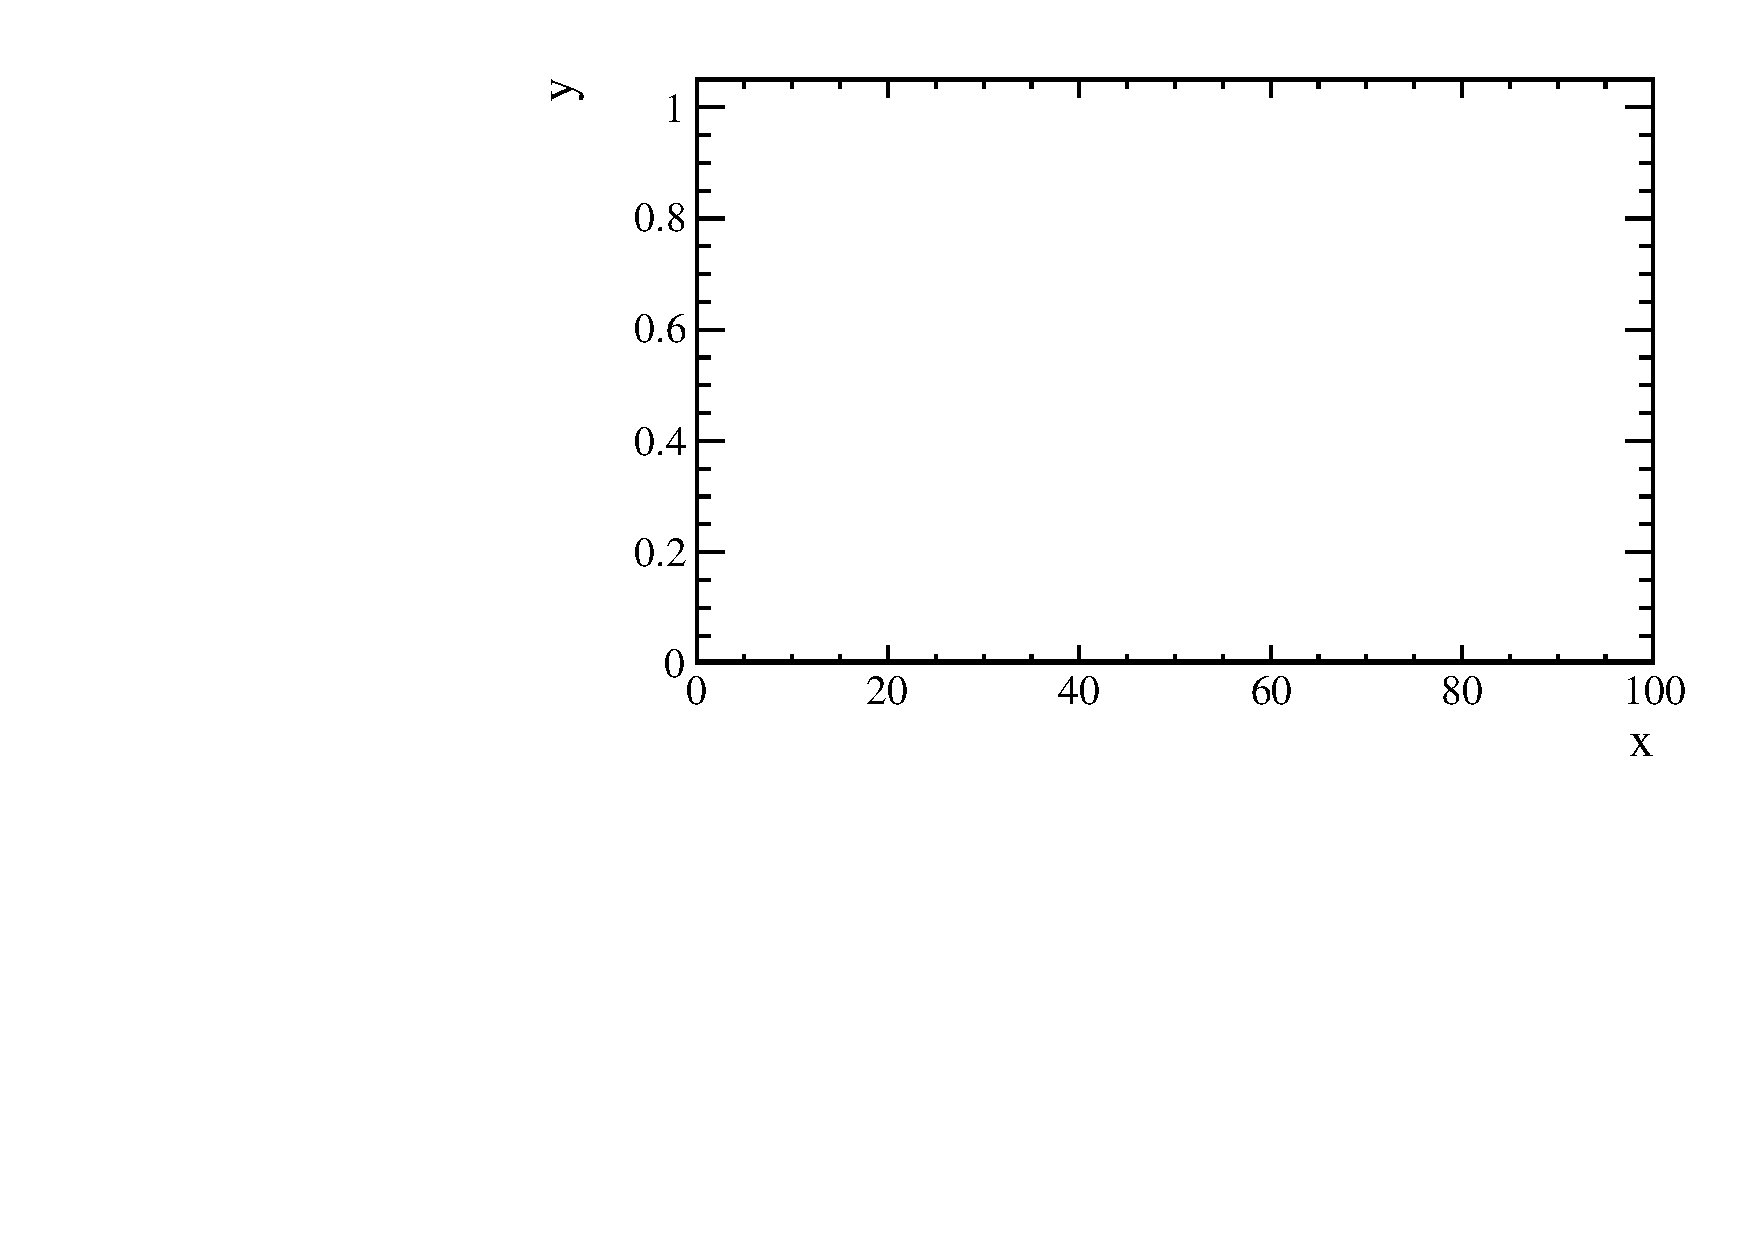
\includegraphics[width=0.48\textwidth]{blank}
    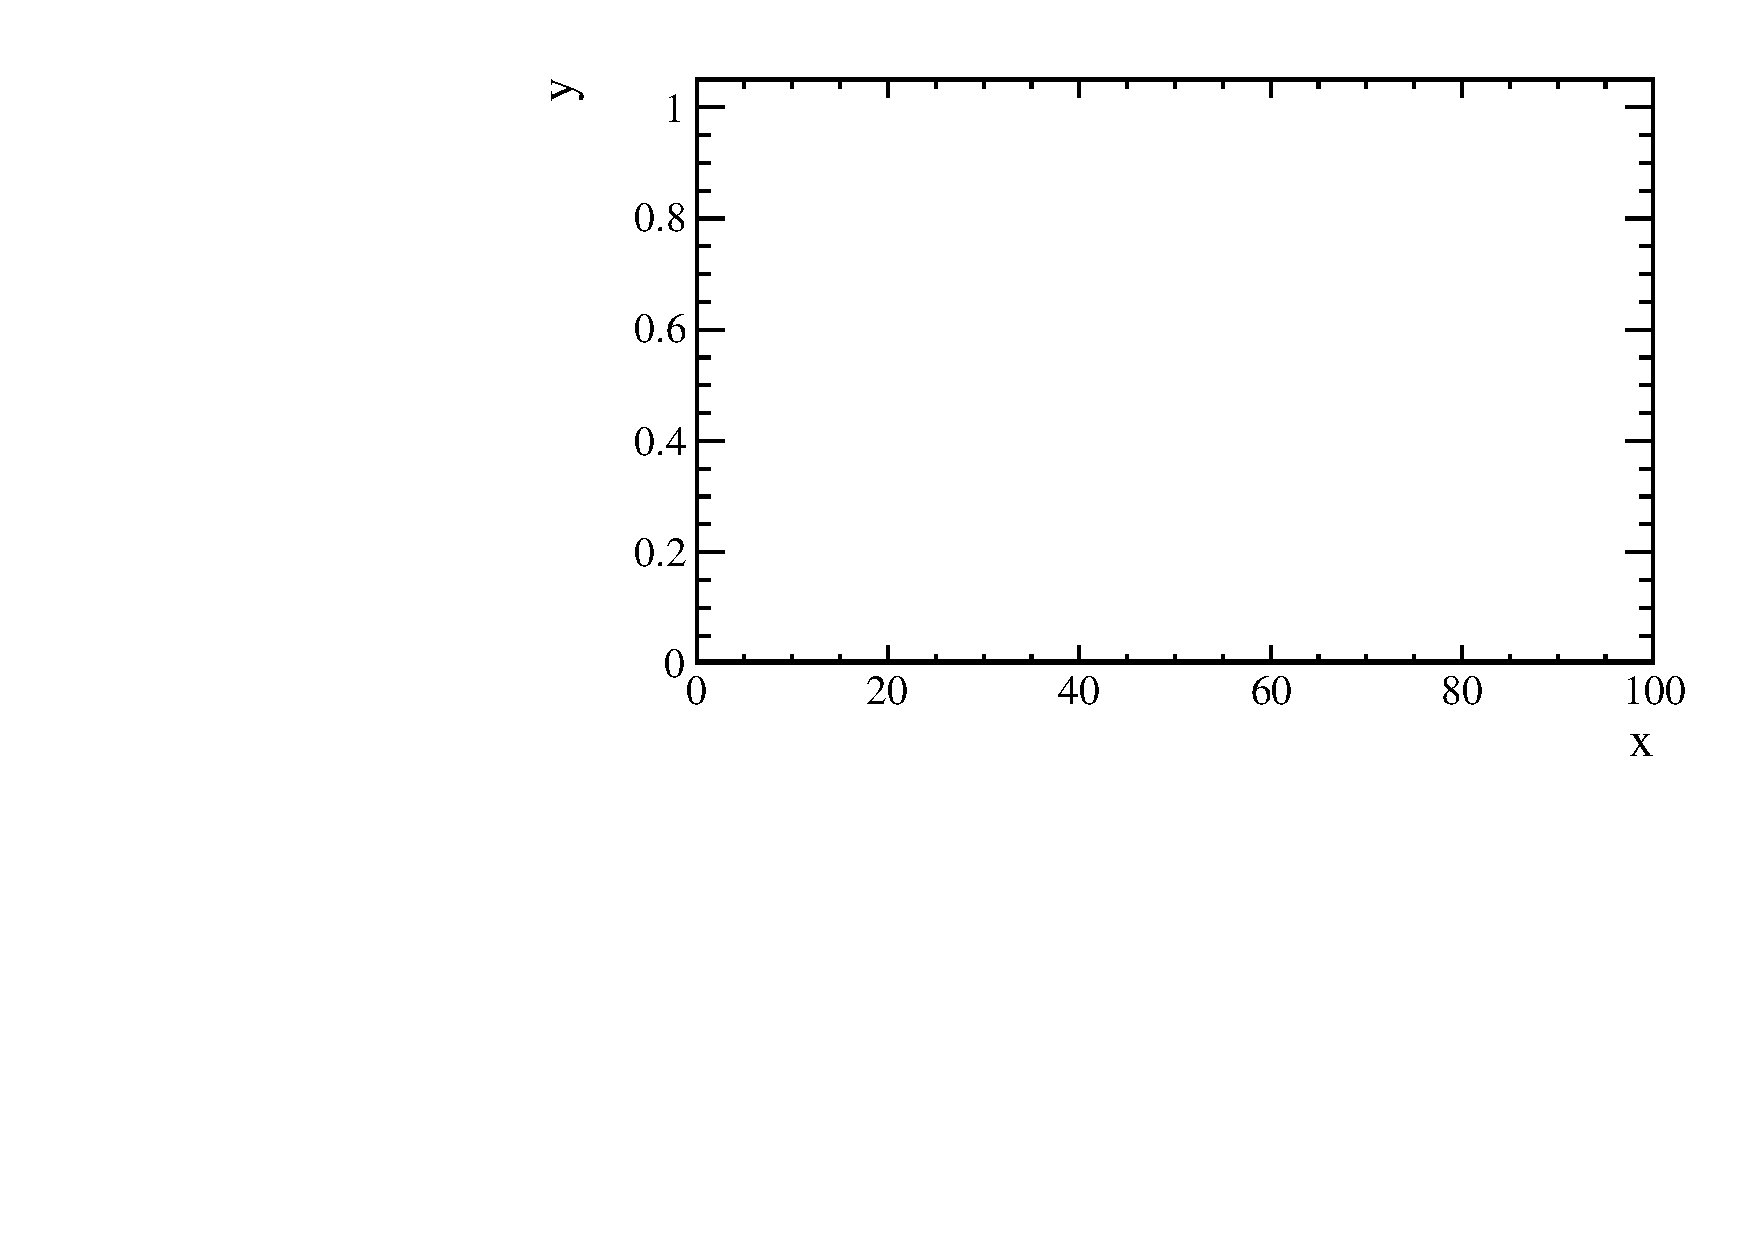
\includegraphics[width=0.48\textwidth]{blank}\\
    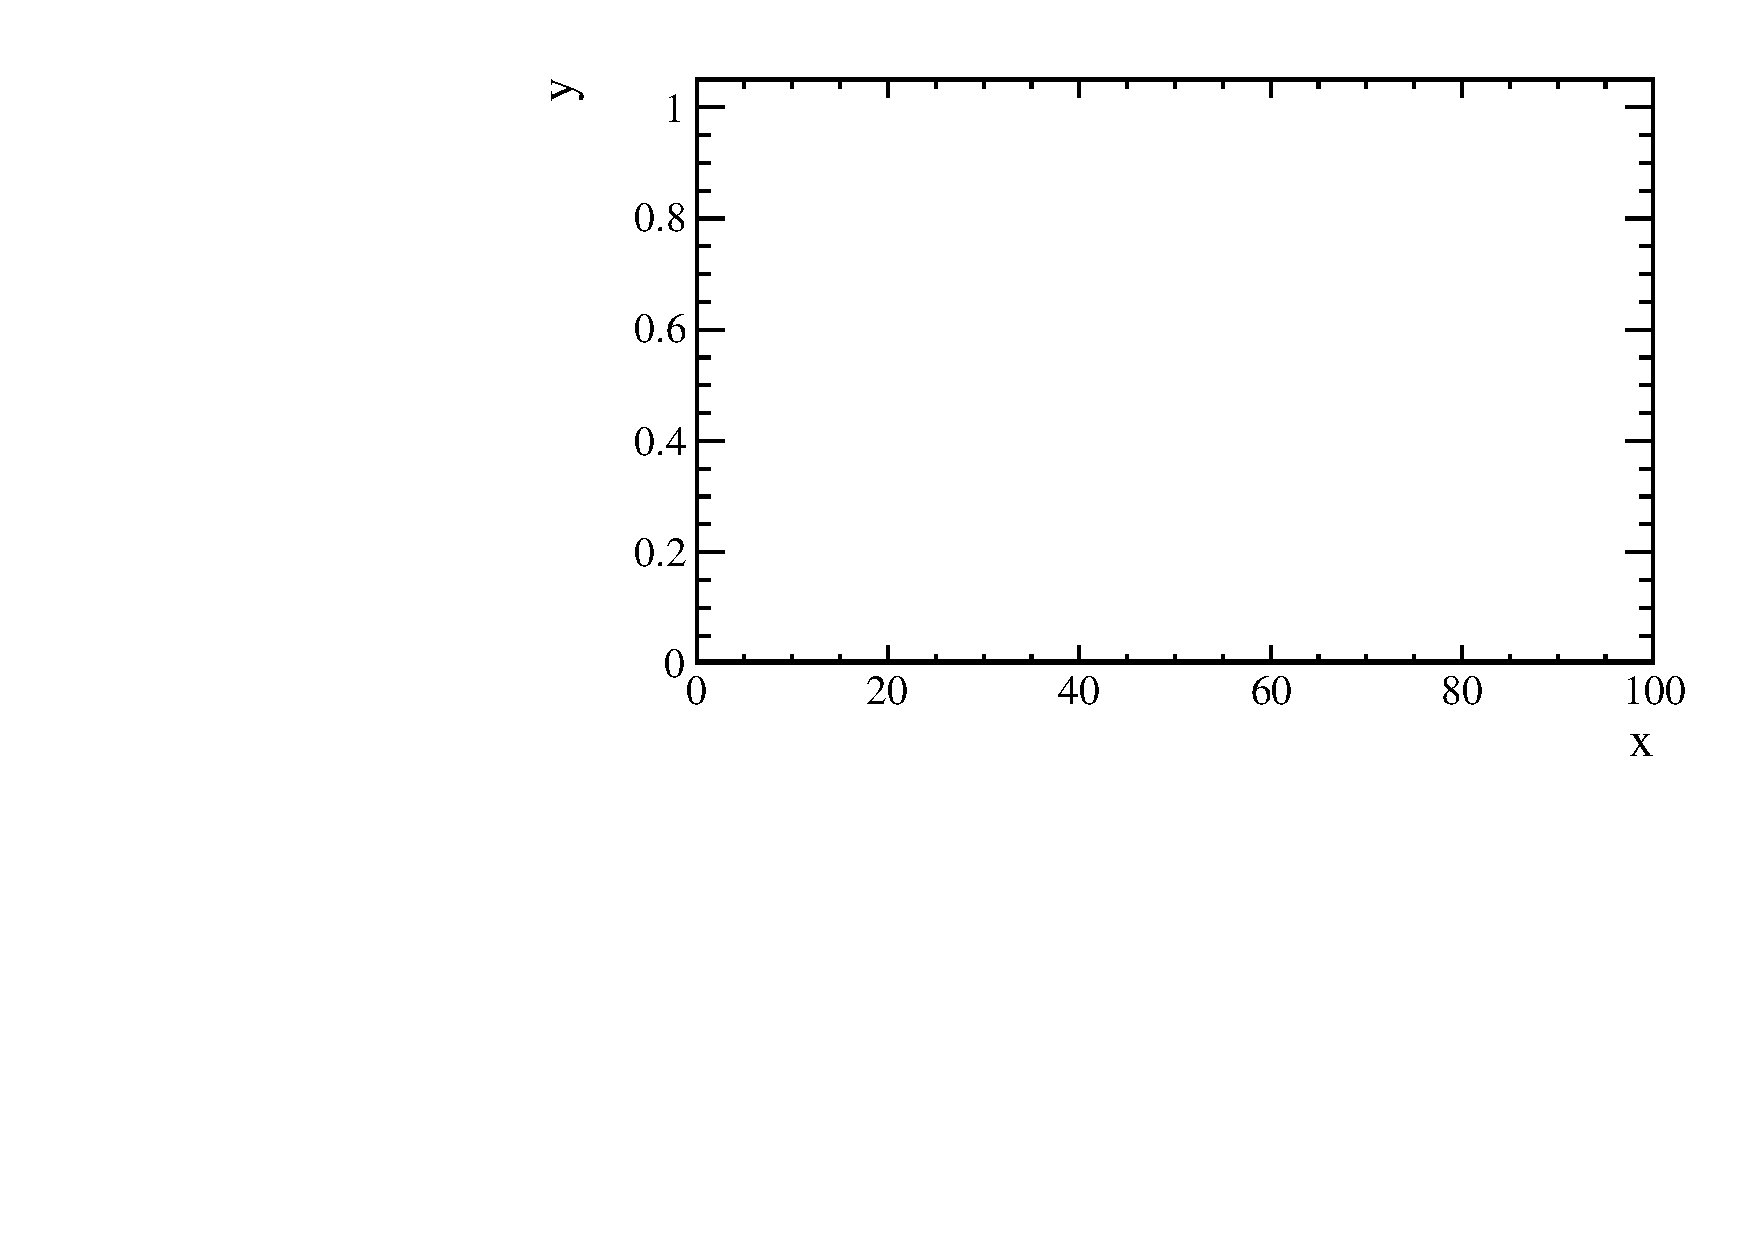
\includegraphics[width=0.48\textwidth]{blank}
    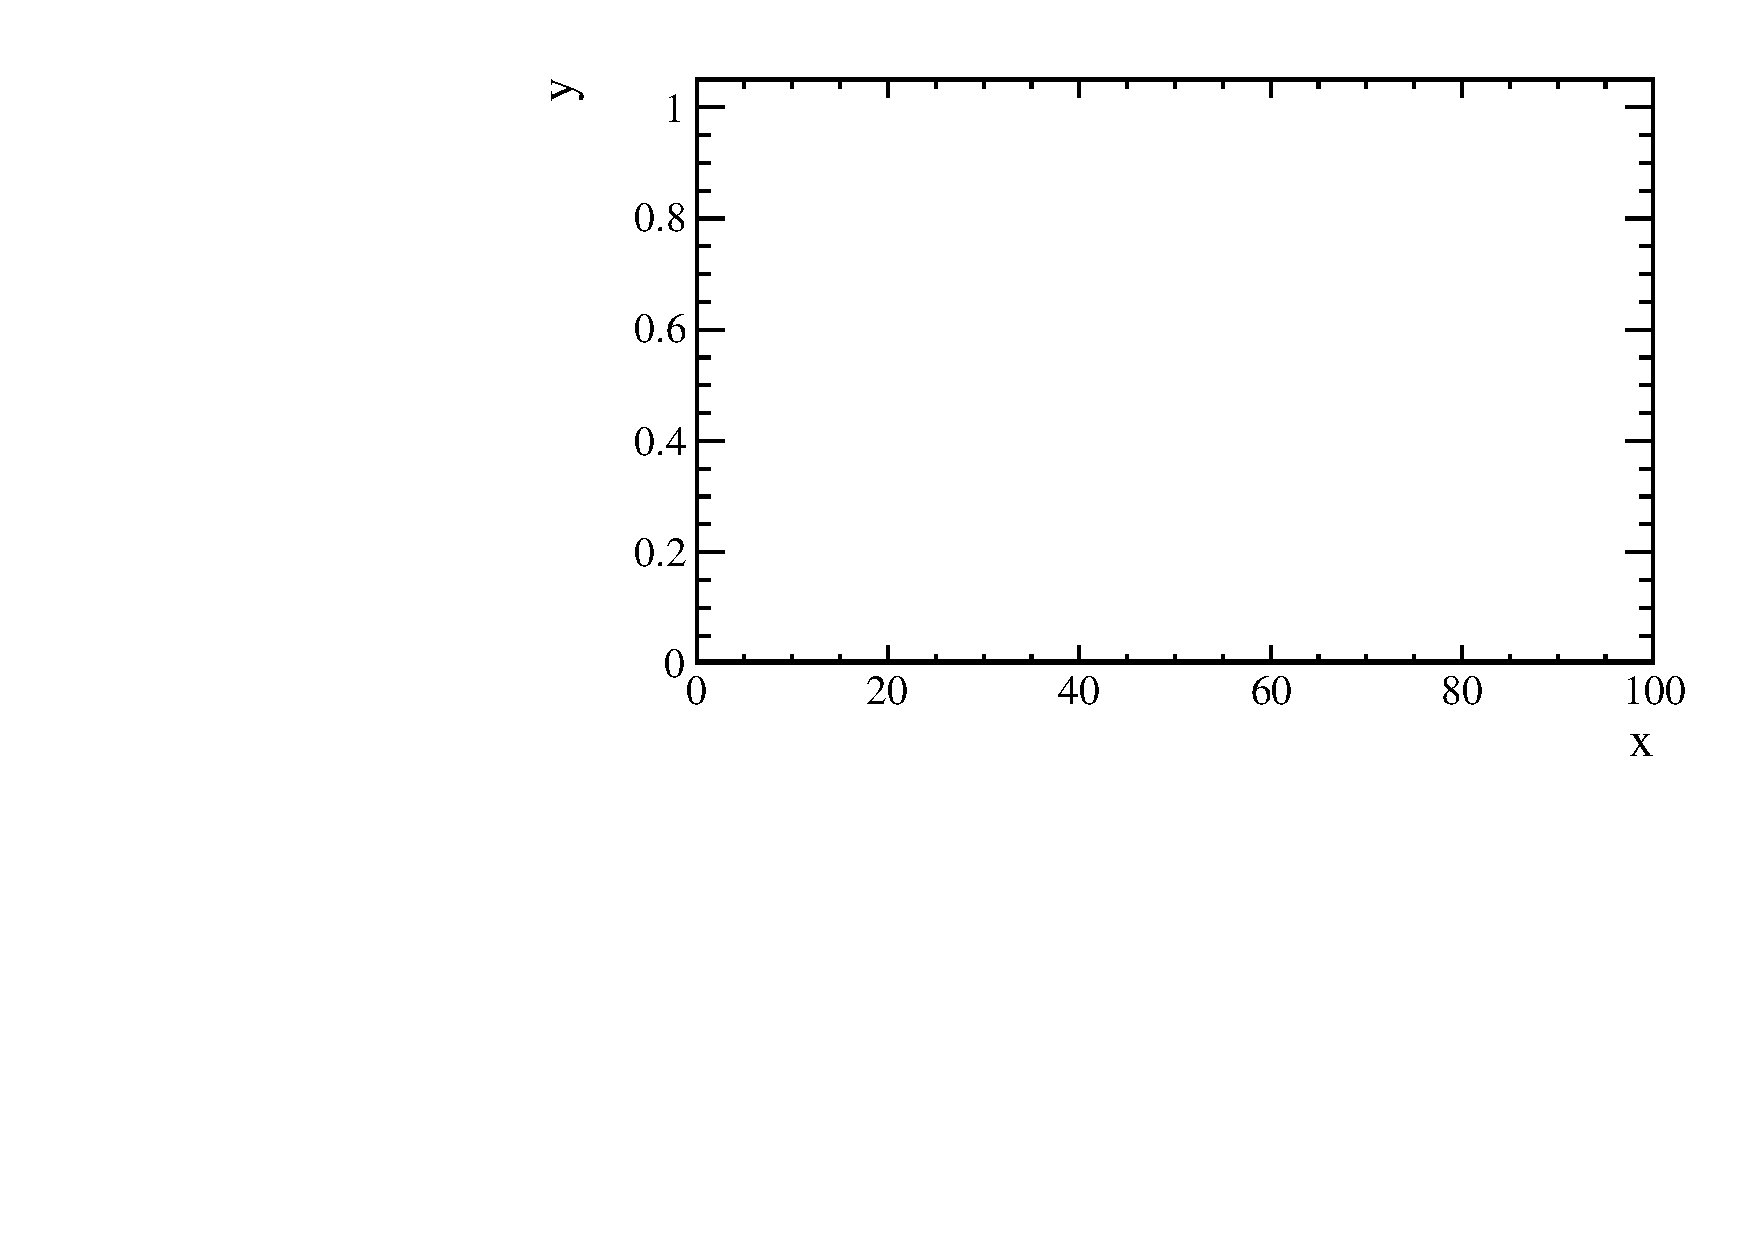
\includegraphics[width=0.48\textwidth]{blank}
    \caption[Shape contributions from signal \btodsphi, and \btodsstrphi]
    {
      Signal shape from simulated events
      Shapes of peaking background contributions for
      decays of the form $\decay{\Bs}{D_s^{(*)+}\Kstarz\Kp}$.
      The contributions from \btodsstrphi and \bstodskstrk are kernelized distributions from
      simulated events.
      The \bstodsstrkstrk shape is obtained by convolving the
      effect of missing a photon or pion with the \bstodskstrk spectrum.
    }
    \label{fig:dsphi:sigshape}
  \end{center}
\end{figure}

It was expected that $\sim7$ events from the decay \btodsstrphi contribute to the background of the
four fit regions, spread over $\sim300\mev$.
At this level, the difference in the true distributions and those shown in \Fig{fig:dsphi:sigshape}
--- especially considering rising shape is the same for all polarizations of the \phii ---
leads to a negligible difference in yield.
For this reason, the longitudinally polarized \btodsstrphi component was used in all regions of the
fit.
The largest uncertainty here was from the yield of this component.
%Far larger, is the systematic effect from the yield.

Just as was done with the signal component, the ratios between yields of each fit region was fixed
using simulation.
Approximately $95\pc$ of the contribution from the decay \btodsstrphi is expected to be in the
signal region.


\begin{figure}
  \begin{center}
    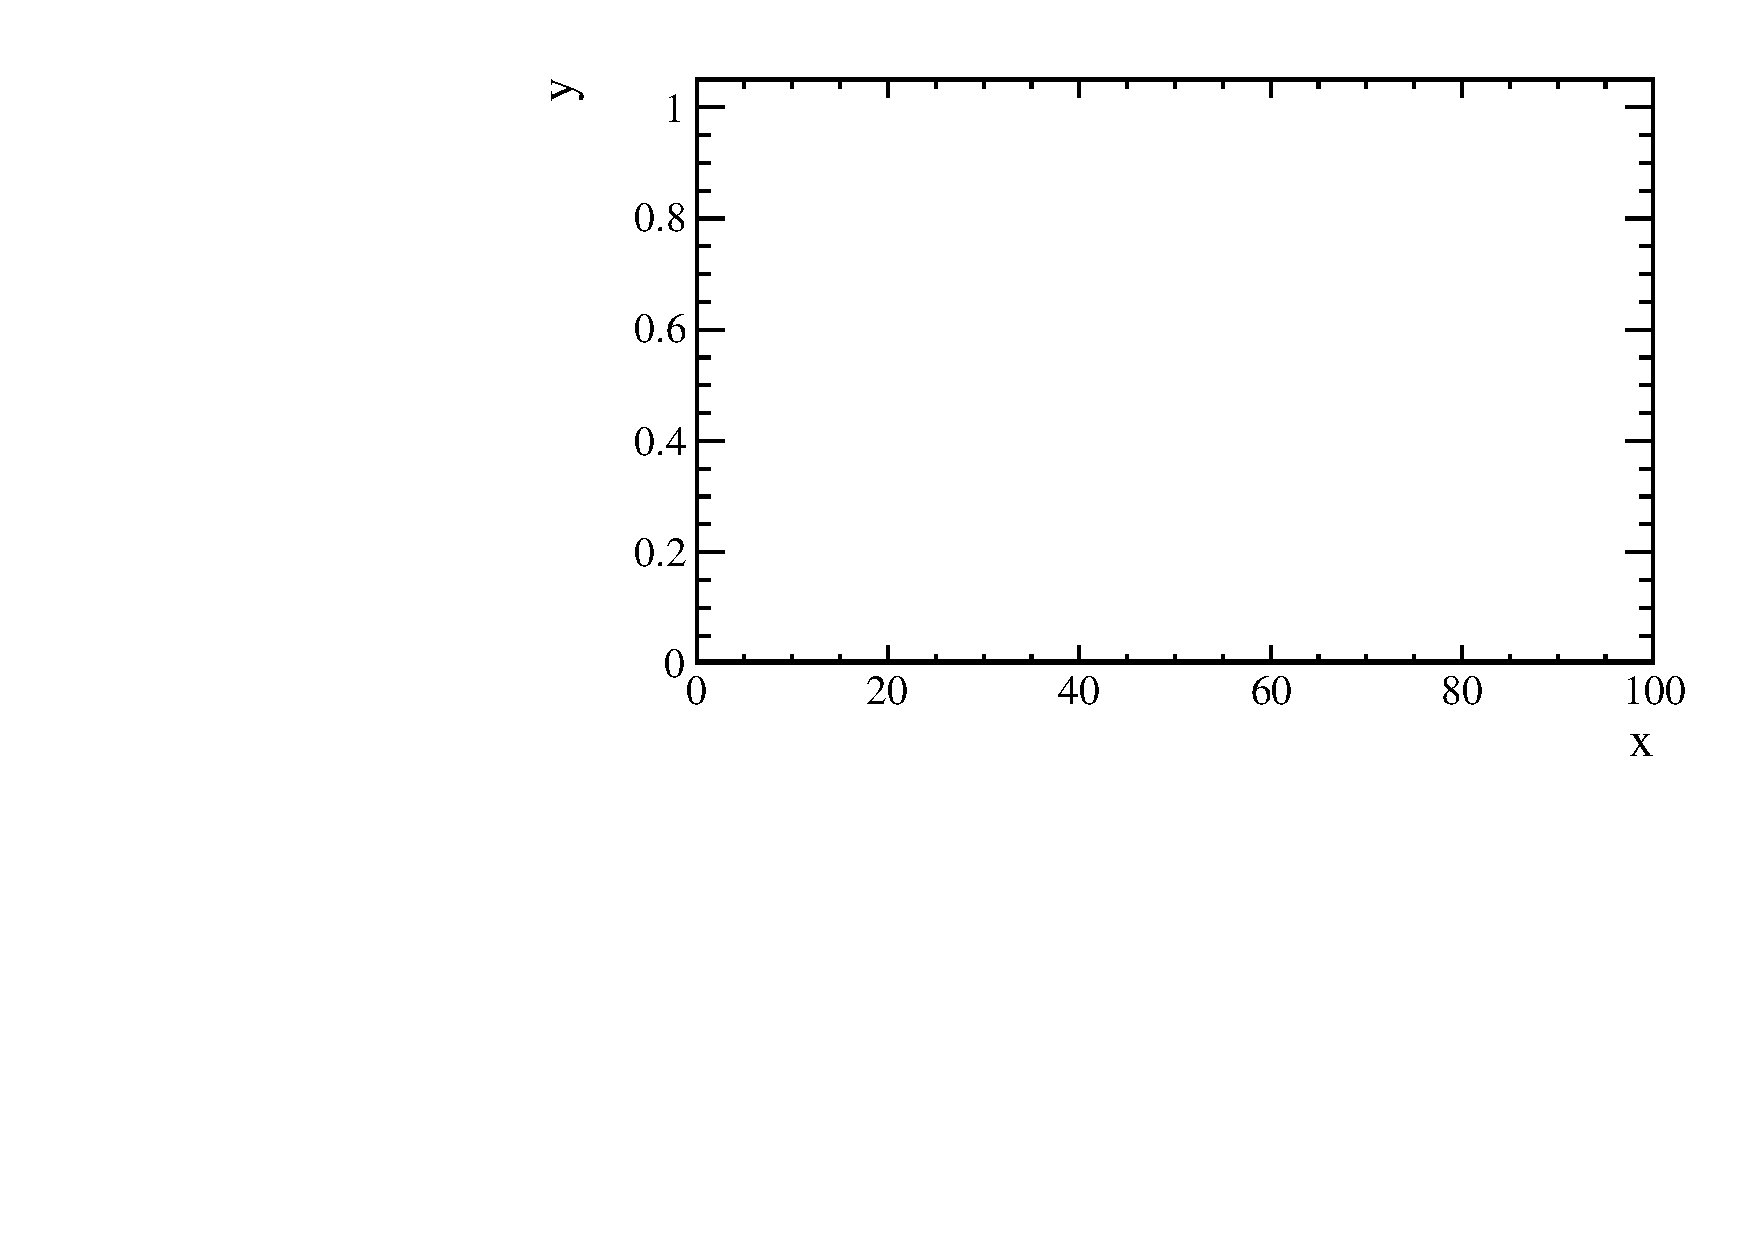
\includegraphics[width=0.48\textwidth]{blank}
    \caption[Shapes of background contributions of \bstodskstrk and \bstodskstrk]
    {\small
      Shapes of peaking background contributions for
      decays of the form $\decay{\Bs}{D_s^{(*)+}\Kstarz\Kp}$.
      The contribution from \bstodskstrk is a kernelized distribution from
      simulated events.
      The \bstodsstrkstrk shape is obtained by convolving the
      effect of missing a photon or pion with the \bstodskstrk spectrum.
    }
    \label{fig:dsphi:bkgshape}
  \end{center}
\end{figure}


%Therefore the value of $\cos\thetahel$ is uniformly
%distributed between zero and one.
%The photon from the decaying \Dssp is not reconstructed, and therefore the background from the
%decay \btodsstrphi peaks below the nominal \Bp mass.


%The decay \btodsstrkstrk has never been observed


Other sources of background that peak below the mass of the \Bp meson are from the decay modes
$\decay{\Bsb}{D_s^{(*)+}\Kstarz\Km}$.
These arise when the pion from the \decay{\Kstarz}{\Kp\pim} is not reconstructed.
Since there is missing energy from the pion (and photon in the case of the \Dssp decay), these peak
significantly below the \Bp mass.
However, their background shapes are non-trivial, extending up to just below the signal window,
and therefore a good understanding of the shapes are required.
Once again, kernel density estimation techniques~\cite{Cranmer:2000du} were used; these shapes are
show in \Fig{fig:dsphi:bkgshape}.

As mentioned previously, the decays \bstodskstrk and \bstodsstrkstrk have never been observed, but
are expected to contribute.
The shape for \bstodskstrk is taken directly from kernelized simulated events.
There were no simulated events available with which to understand the shape of the \bstodsstrkstrk
background.
Instead the shape taken from the \bstodskstrk background is convolved with a distribution
parameterizing the loss of a photon (or pion) as seen between the decays \btodsstrphi and
\bstodskstrk.


Yields from these decays can, clearly, not be estimated.
Especially since the yield from the decay \bstodskstrk is highly sensitive to the width of the
$a_1(1260)$ --- because it decays into $\Kstar K$ --- which is poorly known.
However, the ratios of yields for the \bstodskstrk decay can be determined using simulated events.
The ratios between the yields from \rA/\rB and \rC/\rD was found to be $0.5\pm0.24$, and between the
regions \rA/\rC and \rB/\rD was determined to be $1.50\pm.034$.
These values are used as Gaussian constraints in the fit.
The ratio of branching fractions
\begin{equation}
  \frac{\BF\big(\decay{\Bd}{\Dm\Kstarz\Kp}\big)}
  {\BF\big(\decay{\Bd}{\Dstarm\Kstarz\Kp}\big)}
  \sim 1.5,
\end{equation}
and it is reasonable to expect the same to be true for the branching fraction ratio for the
\bstodskstrk and \bstodsstrkstrk modes.
Therefore, the ration of yields for each region is fixed to $1.5$.

%The background shapes for \btodsstrphi and \bstodskstrk are taken from simulated events,
%reconstructed as \btodsphi candidates.
%Since the shapes of these reconstructed candidates are non-trivial, a

%The shapes of peaking background contributions are taken from kernel density
%estimates of simulated events, as described.
%Yields of background components are also fixed from...
%Therefore, the only floating parameters in the simultaneous fit is the total signal yield and the
%combinatorial background yields and shape.
%However the combinatorial background between regions is fixed.

The last remaining background component to be constrained is that of the combinatorial background,
which is modelled with a decaying exponential function.
Since the distribution of $\cos\thetahel$ is flat for combinations of random tracks, the yields
between the regions \rA/\rC and \rB/\rD  are fixed to $1.5$,
The value of the slope is Gaussian constrained to a fit across a wider range of mass in data.

A summary of constraints applied to the fit is given in \Table{fig:tab:constraints}.

\begin{table}
  \caption[Constraints applied to the fit to \btodsphi data]
  {\small
    Fit parameters used in in the fit to determine the yield of the decay \btodsphi.
    A label of $f$, means that the value is fixed in the fit; and labels of $s$ and $d$ mean
    constrained using simulated events and data over a wider mass range, respectively.
    The yield of the background from \bstodsstrkstrk is also fixed to be $67\pc$ of
    $N\big(\bstodskstrk\big)$
  }
  \label{fig:tab:constraints}
  \begin{center}
    \begin{tabular}{ccccc}
      \toprule
      Fit component & Parameter & Value & Parameter & Value \\
      \midrule
      \btodsphi
      & yield \rA & $6.00\pm2.70$
      & \rC/\rA   & $0.075$ $f$ \\
      & $\mu$     & $5283\mev$ $f$
      & \rB/\rA   & $0.044$ $f$ \\
      & $\sigma$     & $13.2\mev$ $f$
      & \rD/\rA   & $0.003\pc$ $f$ \\
      \midrule
      \btodsstrphi
      & yield \rA & $8.67\pm7.36$
      & \rB/\rA   & $0.044$ $f$ \\
      & \rC/\rA   & $0.00\pm0.12$
      & \rD/\rC   & $0.044$ $f$ \\
      \midrule
      \bstodskstrk
      & yield \rA & $4.94\pm1.29$
      & \rA/\rB, \rC/\rD & $0.50\pm0.24$ $s$ \\
      & \rA/\rC, \rB/\rD & $1.50\pm0.34$ $s$ \\
      %\midrule
      %\bstodsstrkstrk
      %& yield/$N\big(\bstodskstrk\big)$ & 1.5 $f$ \\
      \midrule
      Combinatorial
      & yield \rA & $24.0\pm6.7$
      & yield \rB & $16.5\pm6.0$ \\
      & \rA/\rC & 1.5 $f$
      & \rB/\rD & 1.5 $f$ \\
      & exponent & $-(1.8\pm0.2)\e{-3}$ $d$ \\
      \bottomrule
    \end{tabular}
  \end{center}
\end{table}

Figure~\ref{fig:dsphi:fits} shows the results of the fit of the signal and background functions to
the \btodsphi candidates from data.
The total signal yield gives a value of $N\big(\btodsphi\big)=6.7\,^{+4.5}_{-2.6}$, with a
statistical significance of $3.6\stdev$, as calculated using Wilks Theorem~\cite{wilks1938}.
This is confirmed with an ensemble of $10^5$ toy datasets.

\begin{figure}
  \begin{center}
    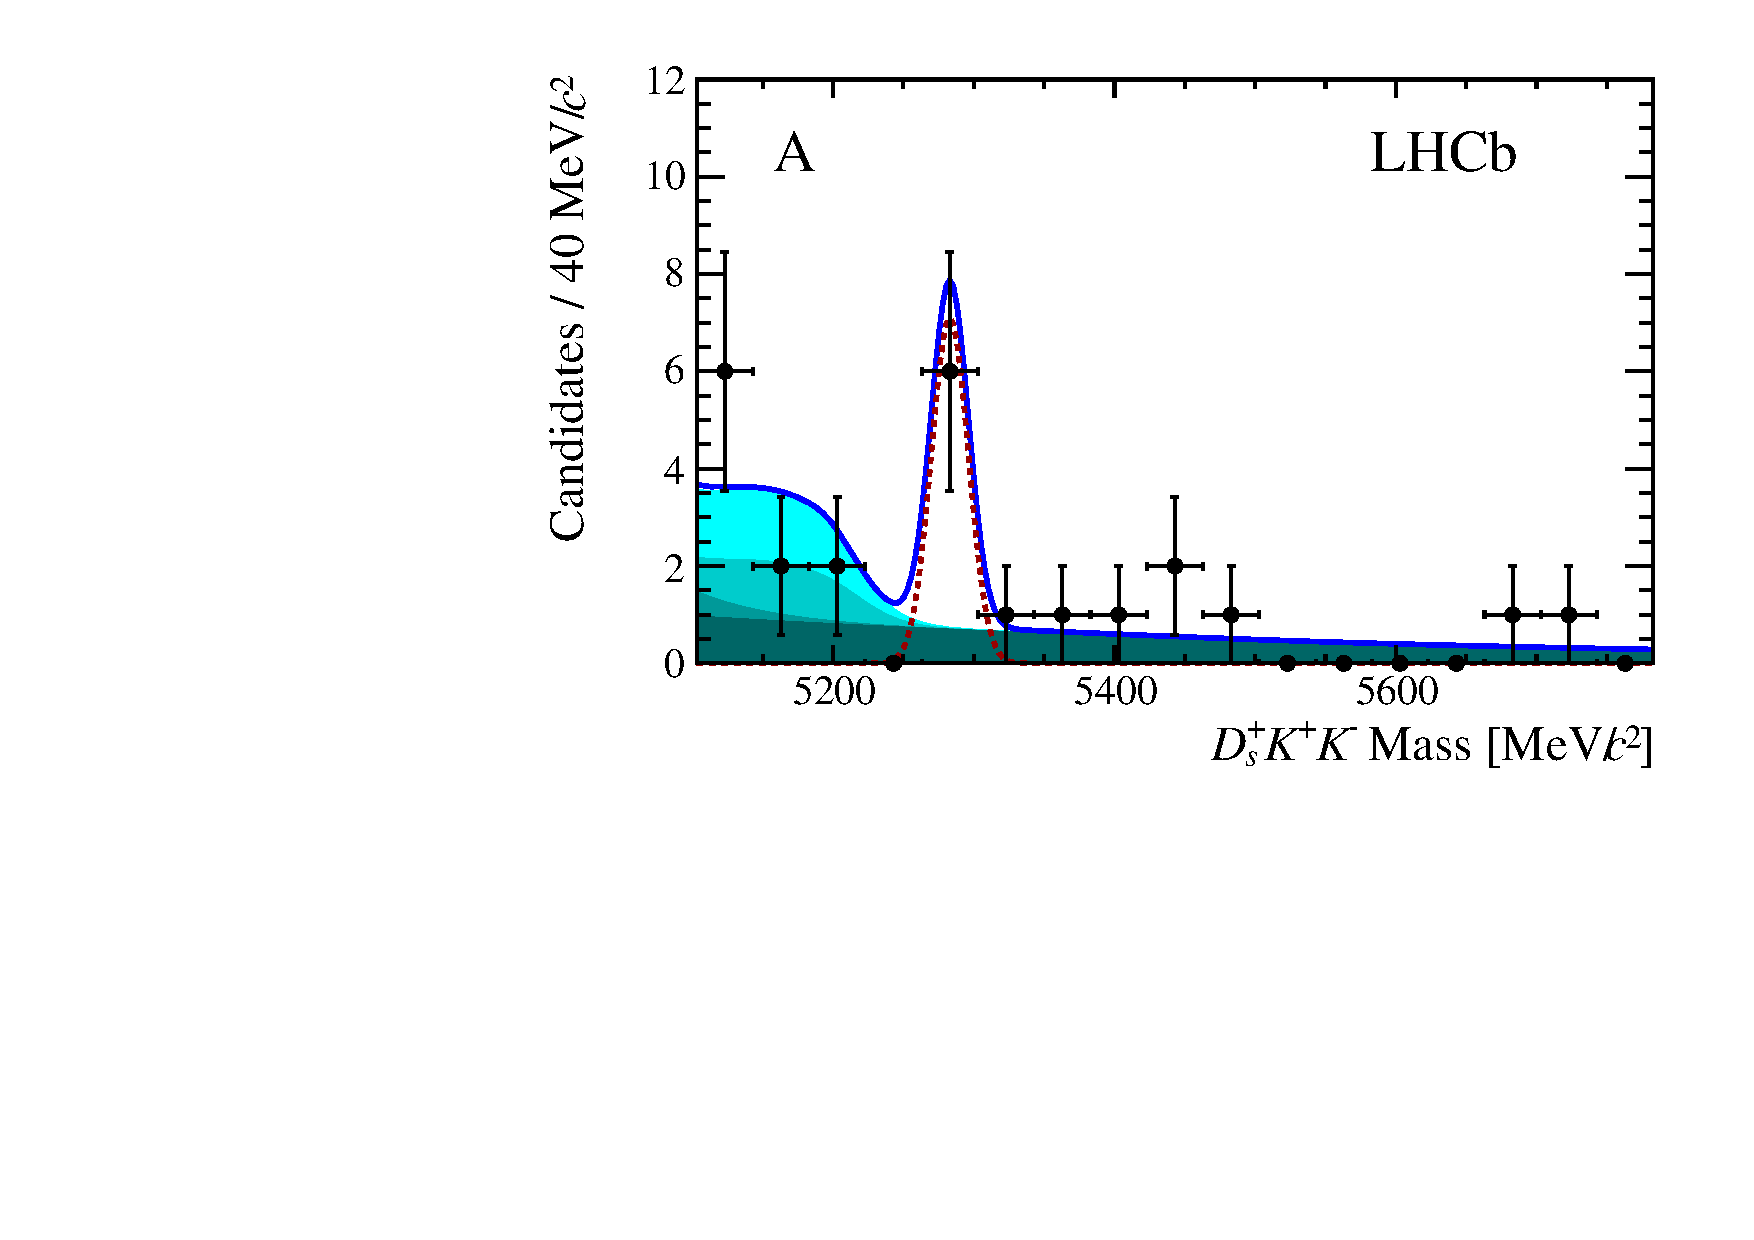
\includegraphics[width=0.48\textwidth]{B2Dsphi_regionA}
    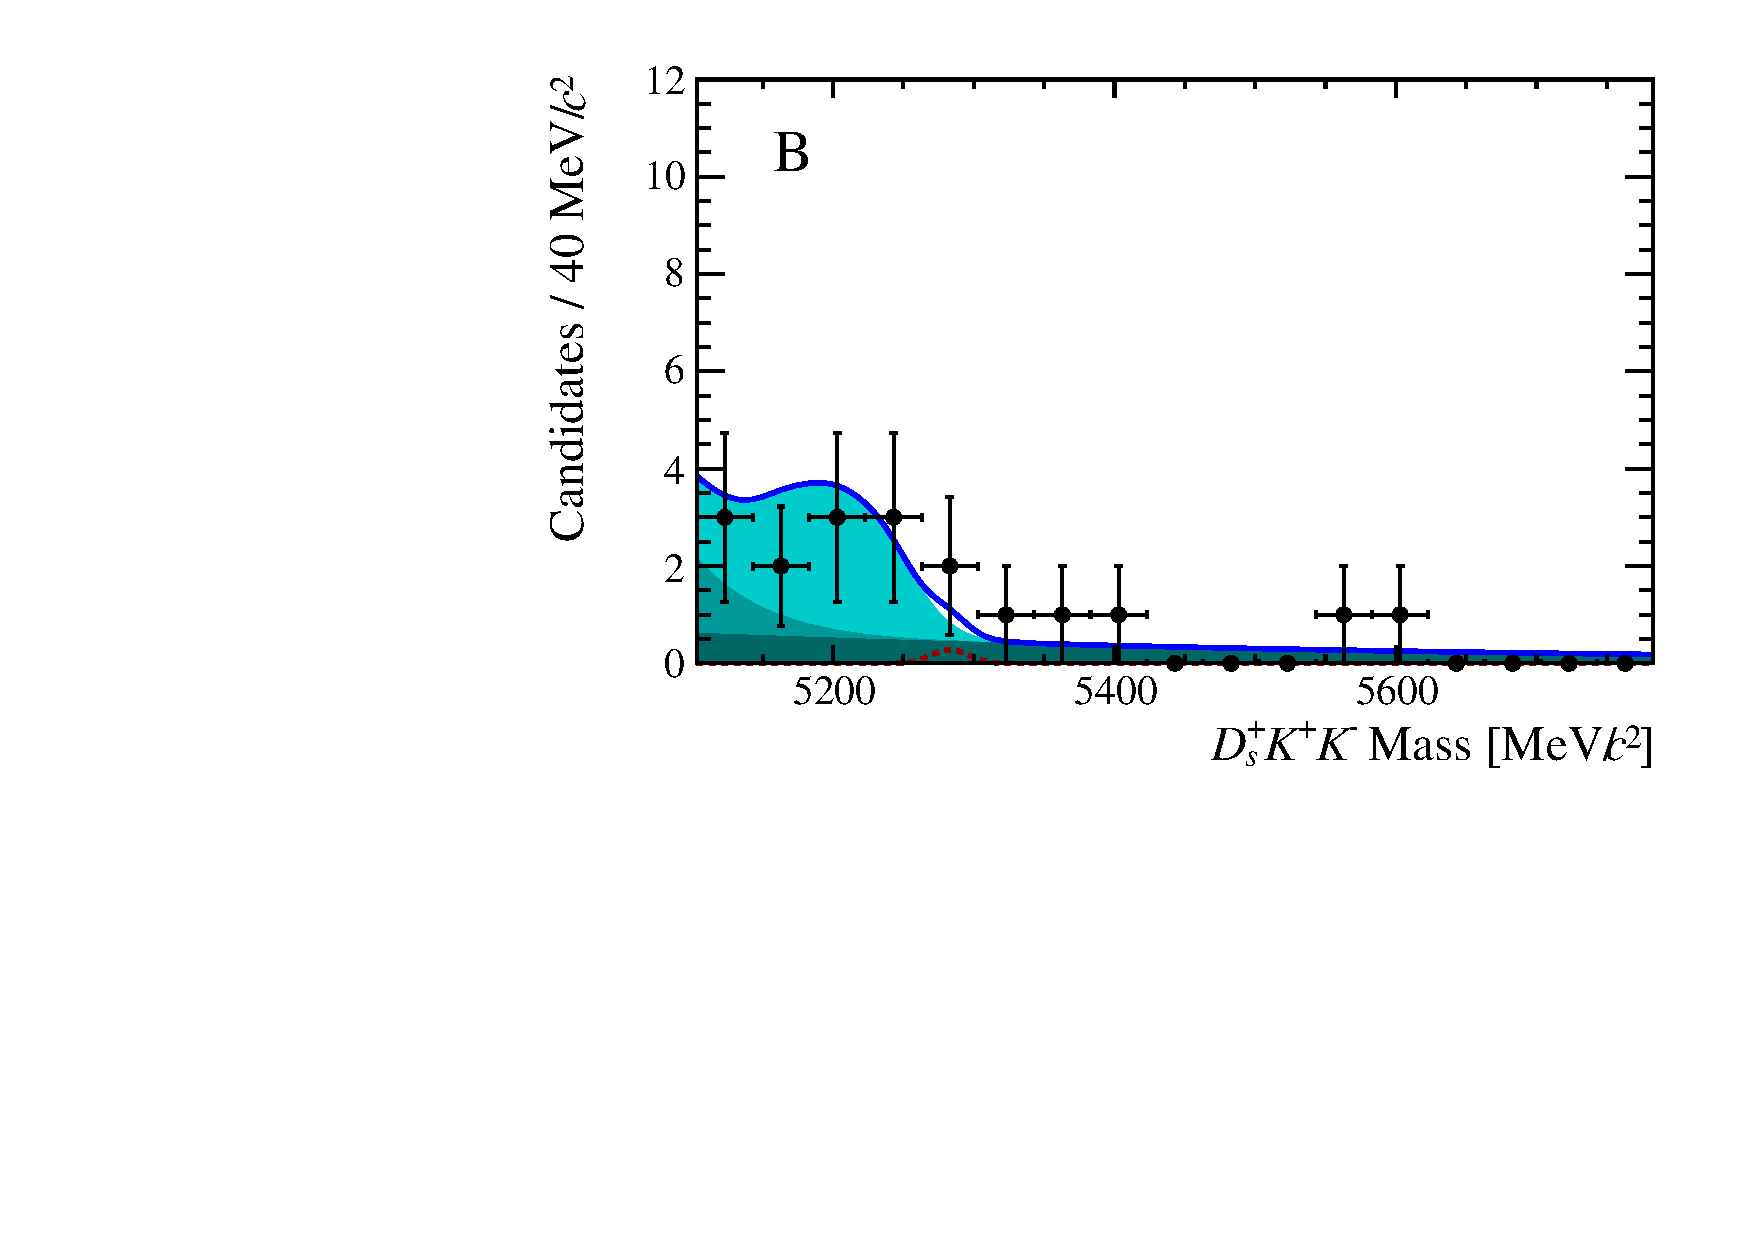
\includegraphics[width=0.48\textwidth]{B2Dsphi_regionB}\\
    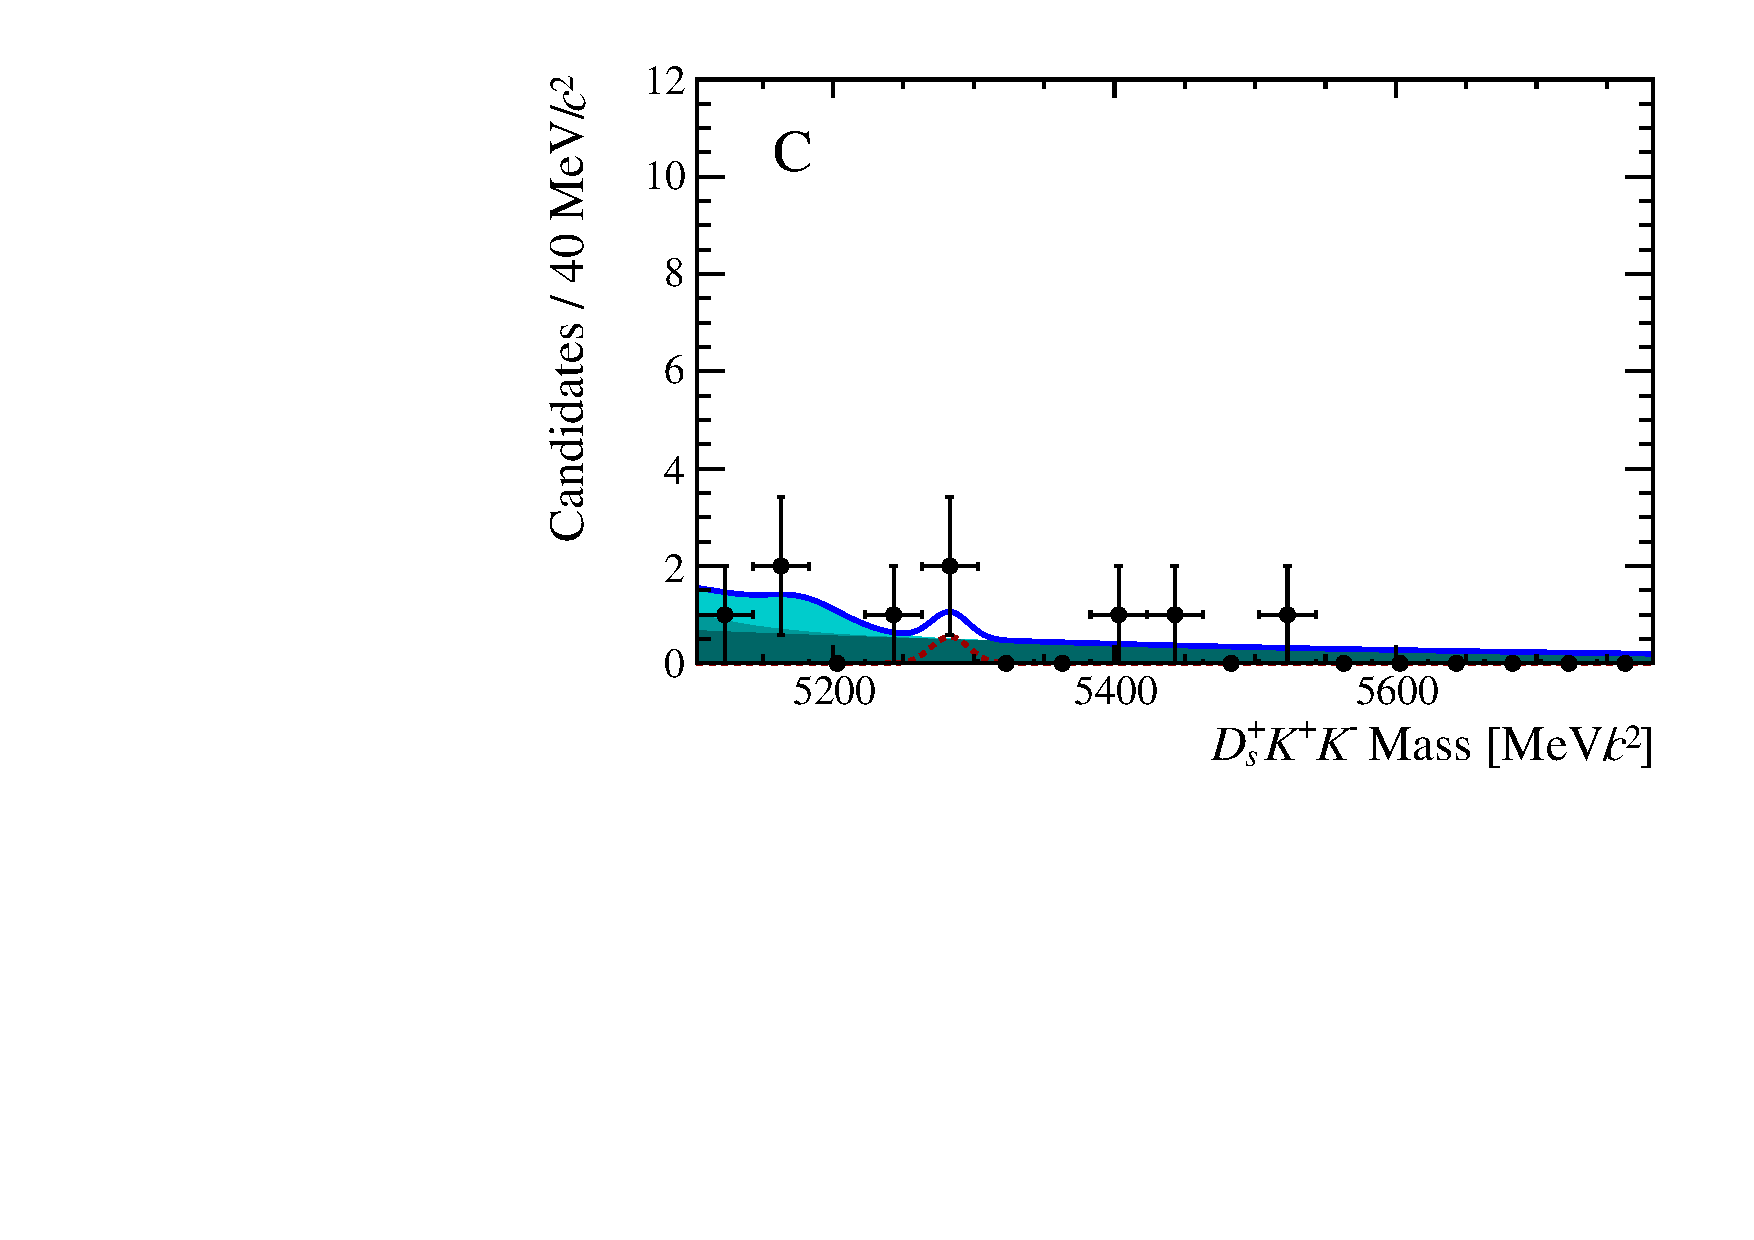
\includegraphics[width=0.48\textwidth]{B2Dsphi_regionC}
    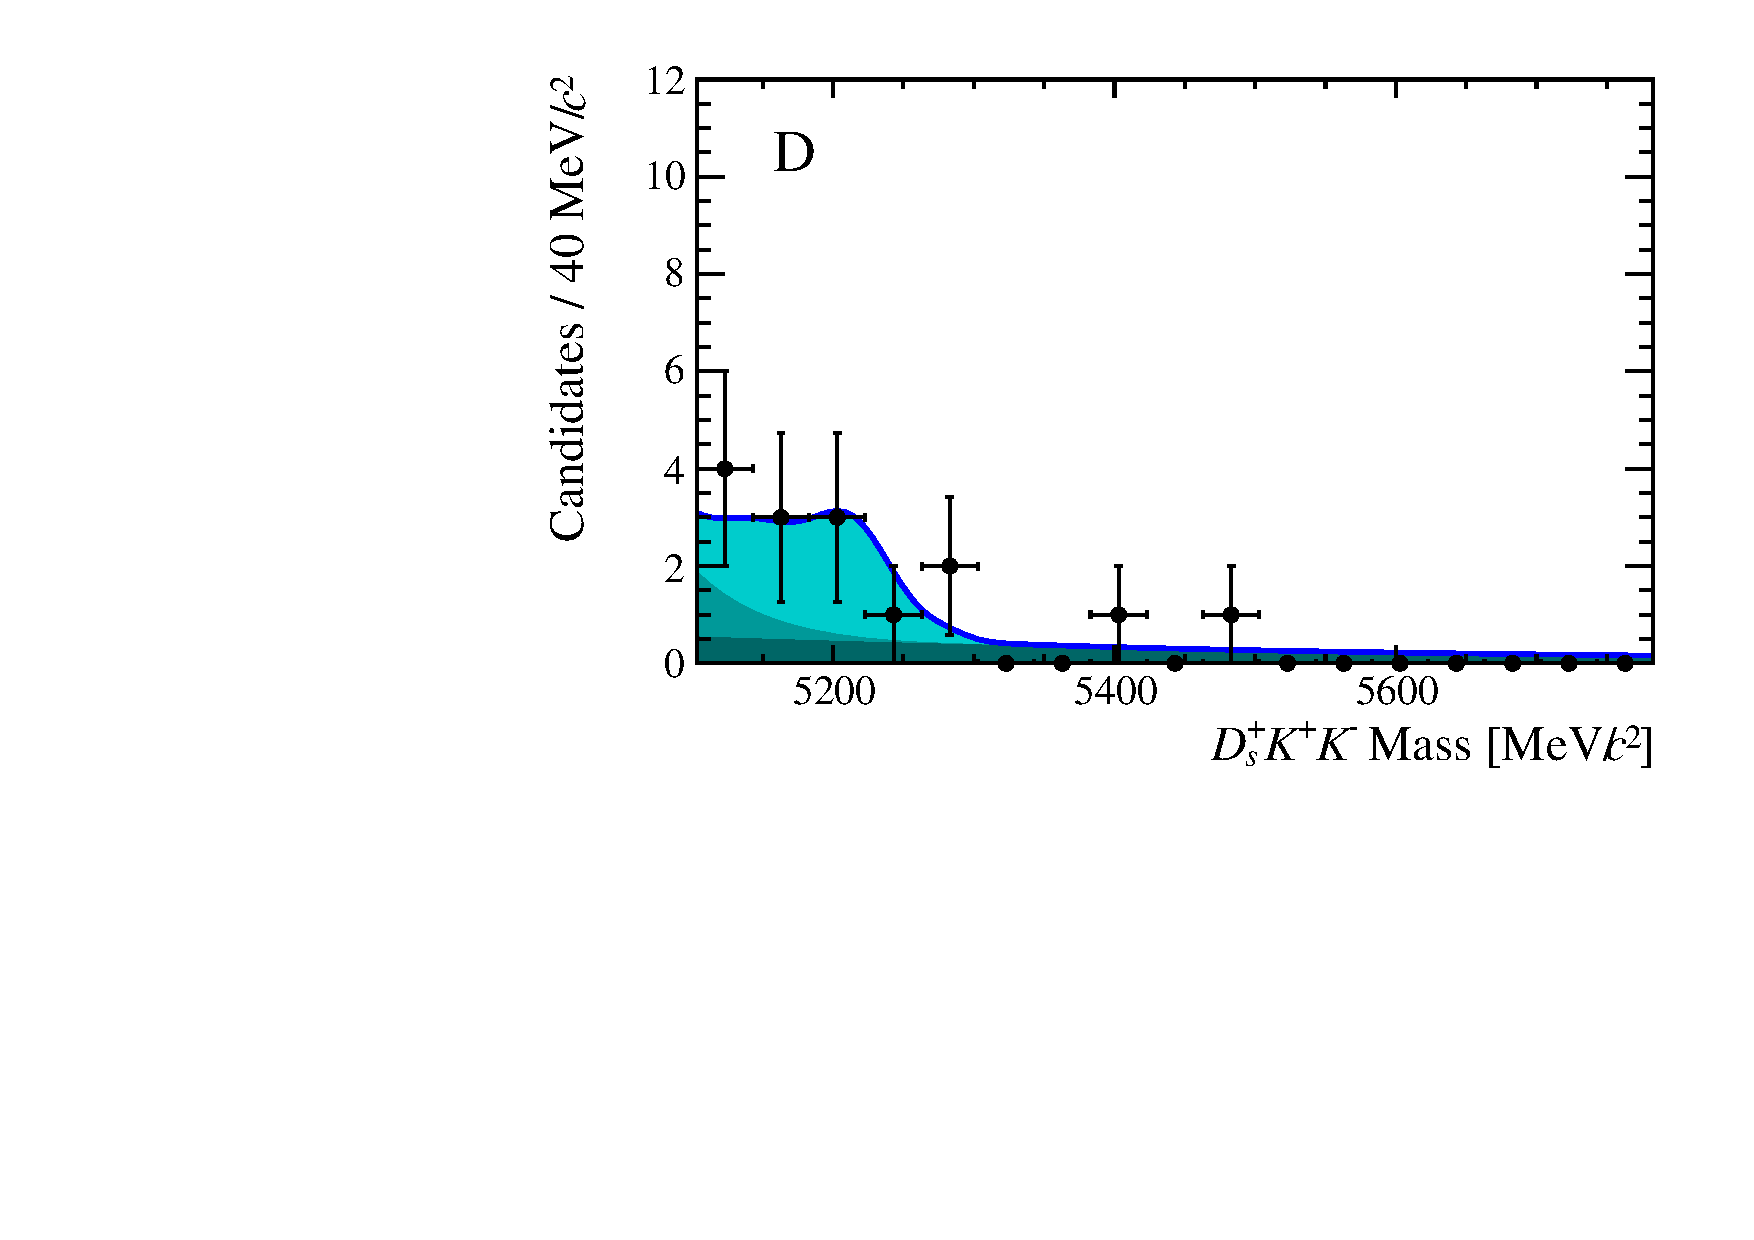
\includegraphics[width=0.48\textwidth]{B2Dsphi_regionD}
    \caption[Fits to \btodsphi data]
    {\small
      Fits to the four analysis regions, as given in Table~\ref{tab:dsphi:hel}, in the search for
      the decay \btodsphi.
      The region \rA is contains the majority of the signal candidates, while region \rD contains
      none.
    }
    \label{fig:dsphi:fits}
  \end{center}
\end{figure}

Using \Eq{eq:dsphi:bf}, the branching fraction of the decay \btodsphi was determined to be
\begin{equation}
  \BF\big(\btodsphi\big) =
  \big(1.87\,^{+1.25}_{-0.73}\stat\pm0.19\syst\pm0.32\normerr\big)\e{-6}.
  \label{eq:dsphi:result}
\end{equation}
This assumes the branching fraction values of
$\BF\big(\btodsd\big)=\big(1.00\pm0.17\big)\e{-2}$,
$\BF\big(\decay{\Dzb}{\Km\pip}\big)=\big(3.88\pm0.05\big)\e{-2}$, and
$\BF\big(\phitokk\big)=\big(48.9\pm0.5\big)\e{-2}$~\cite{PDG2012}.
The uncertainties in the branching fraction of the normalization channel introduced a systematic
uncertainty of $17\ps$.
Other systematic uncertainties are included in the above result, and are discussed in
\Sec{sec:dsphi:syst}.
The above result has a branching fraction which is higher than the SM predictions, although there
are large uncertainties associated with both the theoretical and experimental values.





